\documentclass[aspectratio=169]{beamer}

% ---- packages ----
\usepackage{booktabs}
\usepackage{threeparttable}
\usepackage{graphicx}
\usepackage{amsmath, amssymb}
\usepackage[T1]{fontenc}
\usepackage{lmodern}
\usepackage{adjustbox}

% ---- clean, restrained theme matching the spectrum palette ----
\usetheme{default}
\usecolortheme{default}
\definecolor{interp}{HTML}{1C7293}     % teal-blue
\definecolor{accurate}{HTML}{B85042}   % terracotta
\definecolor{ink}{HTML}{1A2238}        % near-black navy
\setbeamercolor{frametitle}{fg=ink}
\setbeamercolor{title}{fg=ink}
\setbeamercolor{structure}{fg=interp}
\setbeamerfont{frametitle}{series=\bfseries}
\setbeamertemplate{navigation symbols}{}  % no nav clutter
\setbeamertemplate{footline}[frame number]

\title{Method-Agnostic Interpretation via Average Marginal Effects}
\subtitle{Regression-style inference for any supervised model}
\author{Jason Parker}
\institute{Southwest Airlines}
\date{}

\begin{document}
	
	% ============ TITLE ============
	\begin{frame}[plain]
		\titlepage
	\end{frame}
	
	% ============ SLIDE 1: THE SPECTRUM ============
	% Export the spectrum.pptx slide as spectrum.png (or .pdf) and place it
	% in the same directory as this .tex file.
	\begin{frame}{The accuracy--interpretability tradeoff}
		\centering
		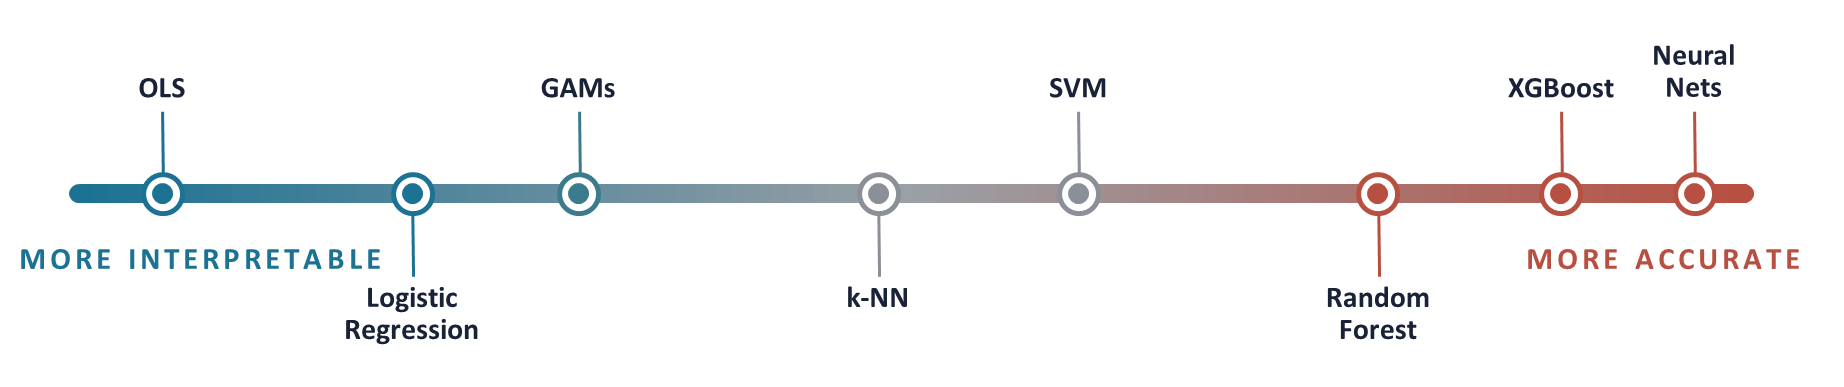
\includegraphics[width=\textwidth]{spectrum.png}
		
		\vspace{0.6em}
		Is the tradeoff really fundamental?
	\end{frame}
	
	% ============ SLIDE 2: THE REVEAL ============
	\begin{frame}{A familiar coefficient table}
		\begin{columns}[c]
			\begin{column}{0.8\textwidth}
				\centering
				\begin{adjustbox}{max width=\textwidth, max totalheight=0.93\textheight}
					\begin{threeparttable}
						\begin{tabular}{lrrrrrrrr}
							\toprule
							& \multicolumn{4}{c}{Logistic} & \multicolumn{4}{c}{XGBoost} \\
							\cmidrule(lr){2-5} \cmidrule(lr){6-9}
							& Spec A & A+B & A+C & A+B+C & Spec A & A+B & A+C & A+B+C \\
							\midrule
							\multicolumn{9}{l}{\textit{Panel A: Demographics}} \\
							\quad age & 0.0060$^{***}$ & 0.0060$^{***}$ & 0.0024$^{***}$ & 0.0027$^{***}$ & 0.0059$^{***}$ & 0.0059$^{***}$ & 0.0029$^{***}$ & 0.0031$^{***}$ \\
							& (0.0001) & (0.0001) & (0.0001) & (0.0001) & (0.0002) & (0.0001) & (0.0001) & (0.0001) \\
							\quad female & -0.1730$^{***}$ & -0.1648$^{***}$ & -0.0275$^{***}$ & -0.0269$^{***}$ & -0.1592$^{***}$ & -0.1446$^{***}$ & -0.0138$^{***}$ & -0.0122$^{***}$ \\
							& (0.0034) & (0.0034) & (0.0041) & (0.0041) & (0.0032) & (0.0032) & (0.0028) & (0.0032) \\
							\quad education\_num & 0.0523$^{***}$ & 0.0393$^{***}$ & 0.0400$^{***}$ & 0.0306$^{***}$ & 0.0610$^{***}$ & 0.0452$^{***}$ & 0.0405$^{***}$ & 0.0312$^{***}$ \\
							& (0.0006) & (0.0007) & (0.0006) & (0.0006) & (0.0023) & (0.0017) & (0.0011) & (0.0011) \\
							\midrule
							\multicolumn{9}{l}{\textit{Panel B: Work Characteristics}} \\
							\quad hours\_per\_week & -- & 0.0048$^{***}$ & -- & 0.0033$^{***}$ & -- & 0.0084$^{***}$ & -- & 0.0032 \\
							& & (0.0001) & & (0.0001) & & (0.0028) & & (0.0025) \\
							\quad government & -- & 0.0029 & -- & 0.0033 & -- & -0.0067$^{*}$ & -- & -0.0003 \\
							& & (0.0051) & & (0.0045) & & (0.0037) & & (0.0026) \\
							\quad self\_employed & -- & -0.0077 & -- & -0.0268$^{***}$ & -- & 0.0113$^{**}$ & -- & -0.0055$^{*}$ \\
							& & (0.0050) & & (0.0044) & & (0.0054) & & (0.0033) \\
							\quad white\_collar & -- & 0.0666$^{***}$ & -- & 0.0541$^{***}$ & -- & 0.0466$^{***}$ & -- & 0.0474$^{***}$ \\
							& & (0.0056) & & (0.0051) & & (0.0026) & & (0.0017) \\
							\quad blue\_collar & -- & -0.0264$^{***}$ & -- & -0.0270$^{***}$ & -- & -0.0446$^{***}$ & -- & -0.0251$^{***}$ \\
							& & (0.0052) & & (0.0048) & & (0.0041) & & (0.0034) \\
							\quad service & -- & -0.0697$^{***}$ & -- & -0.0427$^{***}$ & -- & -0.0807$^{***}$ & -- & -0.0343$^{***}$ \\
							& & (0.0069) & & (0.0066) & & (0.0049) & & (0.0058) \\
							\midrule
							\multicolumn{9}{l}{\textit{Panel C: Financial}} \\
							\quad capital\_gain & -- & -- & 0.0000$^{***}$ & 0.0000$^{***}$ & -- & -- & -0.0001$^{***}$ & -0.0001$^{***}$ \\
							& & & (0.0000) & (0.0000) & & & (0.0000) & (0.0000) \\
							\quad capital\_loss & -- & -- & 0.0001$^{***}$ & 0.0001$^{***}$ & -- & -- & -0.0001$^{***}$ & -0.0000$^{***}$ \\
							& & & (0.0000) & (0.0000) & & & (0.0000) & (0.0000) \\
							\quad married & -- & -- & 0.2854$^{***}$ & 0.2752$^{***}$ & -- & -- & 0.2383$^{***}$ & 0.2357$^{***}$ \\
							& & & (0.0042) & (0.0041) & & & (0.0035) & (0.0036) \\
							\midrule
							McFadden $R^2$ & 0.199 & 0.233 & 0.376 & 0.400 & 0.257 & 0.296 & 0.467 & 0.492 \\
							Accuracy & 0.797 & 0.806 & 0.841 & 0.847 & 0.805 & 0.818 & 0.864 & 0.872 \\
							\bottomrule
						\end{tabular}
						\begin{tablenotes}
							\footnotesize
							\item \textit{Notes:} Average marginal effects on $P(\text{Income} > \$50\text{k})$. $^{***}p<0.01$, $^{**}p<0.05$, $^{*}p<0.10$. Bootstrap standard errors (200 replicates) in parentheses.
						\end{tablenotes}
					\end{threeparttable}
				\end{adjustbox}
			\end{column}
			
			\begin{column}{0.2\textwidth}
				\raggedright
				{\color{accurate}\bfseries The right four columns are XGBoost.}\\[0.6em]
				{\color{ink}\small Same table you already read --- estimates, standard errors, significance --- for a black-box model.}
			\end{column}
		\end{columns}
	\end{frame}
	
	% ============ FRAMING / REASSURANCES ============
	% This slide is mainly for the version that gets forwarded up the chain.
	% You can skip past it when presenting live.
	\begin{frame}{What this is}
		\begin{itemize}
			\item A method for reading \textbf{any} machine learning model as a regression-style coefficient table --- estimates, standard errors, significance.
			\item Distilled from a full-length companion manuscript (105 pages, complete proofs); a condensed 10-page version is the conference submission.
			\item Built entirely on \textbf{my own time}, using \textbf{public datasets} only, with \textbf{no Southwest data} or proprietary information.
		\end{itemize}
	\end{frame}
	
\end{document}